% !TEX root = ../main.tex
\section{The History of Graphical Passwords} \label{sec:historygraphicalpasswords}
	 
  This section will review related work on graphical passwords from a historical point of view. The graphical password schemes reviewed will provide an elaboration of how the scheme works as well as a graphical illustration of its design. Like text-based passwords schemes, graphical password schemes are also a knowledge-based authentication scheme, e.g. ``something you know''. Since it all started around 1996, there have been many suggestions for graphical password schemes. When a new password scheme is proposed, there are several aspects of password that needs to be considered. A password scheme needs to be secure in terms of entropy, and it needs to be hard to guess, and it also needs to be comfortable to use. The history of graphical passwords are important to know because each scheme is trying to improve different aspects of earlier graphical password. Looking at graphical passwords from a historical point of view can give us a detailed understanding of today's situation. The review starts by looking at where the first graphical passwords originated from ending with looking at todays situation of graphical passwords.

  Greg Blonder initially described the idea of graphical passwords in a patent published in 1996 \cite{Blonder}. The graphical password scheme proposed was requiring the user to tap on a selection of points on a predefined image in order to pass the authentication process. This was just a proposal, and did not further explore the power of graphical passwords, nor analyzed the security aspects of the proposal. Figure \ref{fig:blonder} is a picture from Blonder's patent of the first graphical password scheme.

    \begin{figure}[H]
      \centering
      \subfigure[Proposal for a graphical password scheme\cite{Blonder}]{
        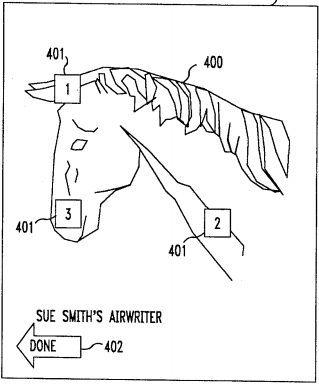
\includegraphics[width=0.30\textwidth]{pics/review/blonder.png}
        \label{fig:blonder}
      }
      \subfigure[DAS \cite{Jermyn}]{
        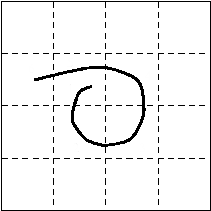
\includegraphics[width=0.30\textwidth]{pics/review/DAS.png}
      \label{fig:DAS}
      }
      \subfigure[BDAS \cite{BDAS}]{
        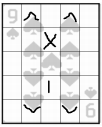
\includegraphics[width=0.30\textwidth]{pics/review/BDAS1.png}
        \label{fig:BDAS}
      }
    \end{figure}

  In 1999, Jermyn et al. \cite{Jermyn} suggested a new graphical password scheme called Draw-a-secret (abbreviated DAS). DAS was the first recall-based graphical password scheme proposed. The motivation for the graphical password scheme was that graphical input devices enables the user to decouple the position of inputs from the temporal order in which they occur, and shows that the decoupling can be used to generate passwords that have a larger and more memorable password space. In order to make a more memorable password, the research group argued that the DAS was more secure than text-based passwords because the users were able to remember longer and more complex passwords. After the DAS scheme was published, Dunphy and Yan \cite{BDAS} added an extra background image to the DAS and named it "Background DAS" (BDAS). The thought behind adding an background to the DAS was to encourage their users to make more complex passwords. Dunphy and Yan believed that the extra image would support the users to remember longer and more complex passwords, and therefore stating that the BDAS was more secure than DAS. Figure \ref{fig:DAS} and Figure \ref{fig:BDAS} are showing images of the DAS and the BDAS respectively.

  In 2000, Dhamija and Perrig \cite{DejaVu}, created a new password scheme called ``Deja Vu''. The password scheme was based on the hash visualization technique \cite{HashVisualization}, a technique that replaces meaningless strings with structured images. The structured images are looking like random art because they are created out of the bits from the meaningless string. Dhamija and Perrig wanted to make a graphical password scheme that solved some of the shortcomings with recall-based authentication like PIN's and text-based passwords. Deja Vu should purely rely on recognition rather than recall, and it should be hard to write down and share the password with others. The randomly generated pictures, based on the hash visualization technique, makes it hard to share the password since the images is hard to recreate but are easy to remember. Instead of writing your own art on a grid, the users are asked to select a sequence of images from a random set of images that are generated by the hash visualization technique. Figure \ref{fig:DejaVu} are showing the Deja Vu where the hash visualization technique are for generating images from random strings looking like random art.

    \begin{figure}[H]
      \centering
      \subfigure[Passfaces \cite{passface}]{
        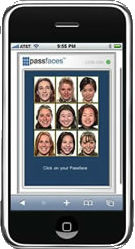
\includegraphics[scale=0.7]{pics/review/Passfaces.jpg}
        \label{fig:Passfaces}
      }
      \subfigure[DejaVu \cite{DejaVu}]{
        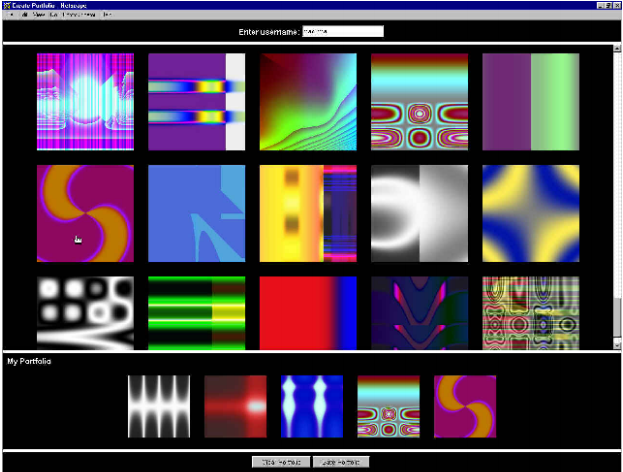
\includegraphics[scale=0.37]{pics/review/DejaVu1.png}
        \label{fig:DejaVu}
      }
    \end{figure}  

  ``Passfaces'' is a graphical password scheme developed by Real User Corporation that was founded in 2000 \cite{passface}. The Passfaces scheme asks the user to first select four images that are a visualization on human faces. The four faces selected represent the password, and the user get authenticated by identifying the four selected faces. The selected faces will be shown together with 8 other faces that is not included in their own selected faces. The scheme exploits the advantage that people are good at recognizing people, so when users choose the human faces they can use the characteristics of the human faces in the process of remembering their password. Passfaces are quite similar to the previous described scheme Deja Vu. The major difference between the schemes are that they are using different association elements in the images, faces and random art. Figure \ref{fig:Passfaces} is showing the PassFaces scheme used on a smartphone. This is one of the few commercial graphical password schemes that are in use. 

  Passdoodle was a new scheme first purposed by Goldberg et al. in 2002 and later studied by Varenhorst in 2004 \cite{PassDoodle,Varenhorst}. The Passdoodle is similar to DAS, but allows users to create a freehand drawing as a password, but uses a more complex matching process without the visible grid. To add variability to the doodles, additional characteristics like color, drawing speed, and number of pen strokes, have been suggested. Figure \ref{fig:doodle} is an example of a freehand drawn doodle.

  In 2004, Davis et al. did a comparison of a light version of ``PassFace'' and a new graphical password scheme called ``Story'' \cite{Davis}. The Story scheme is making the users choosing images to make up a story instead of just recalling a set of faces. Story was created to help users remembering their passwords by making a memorable story of images. In order to pass the authentication, the story had to be recalled in the correct order. To support the memorability, users were instructed to construct a story mentally to connect the everyday images in the set. Figure \ref{fig:story} is an image of Story scheme showing the images of objects used to create a story.

  
  In 2005 Wiedenbeck et al. proposed a graphical password scheme called ``PassPoints'' \cite{Wiedenbeck2} that is an  extension of the Blonder's \cite{Blonder} idea by eliminating the boundaries and allowing arbitrary images to be used. They evaluated their password scheme by testing the scheme for human users. The results showed that PassPoint were a promising scheme with respect to memorability because of the low error rate and low clicking rate. The aim of this study was to get an understanding of how different images affected user performance in authentication with a graphical password scheme. The preliminary result showed suggested that images may support memorability in graphical password schemes. Figure~\ref{fig:passpoints} is an image of the PassPoints scheme.
  \todo{Skrive om dette. Flytte til 4.2?}

    \begin{figure}[H]
      \centering
      \subfigure[Story \cite{Davis}]{
        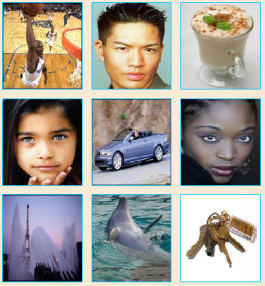
\includegraphics[scale=0.4]{pics/review/story.png}
        \label{fig:story}
      }
      \subfigure[PassPoints \cite{Wiedenbeck2}]{
        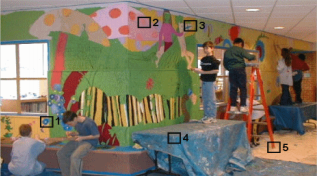
\includegraphics[scale=0.65]{pics/review/passpoint.png}
        \label{fig:passpoints}
      }  
    \end{figure}

  In 2006, a research group wanted to address the problem with graphical passwords and the shoulder surfing problem. They called their password scheme ``Convex Hull Click'' (abbreviated CHC) \cite{Wiedenbeck}. The CHC allows the user to use the scheme in secure and insecure locations because because users do not directly click on the images in the password. This design makes it hard for attackers to perform a shoulder surfing attack. In CHC has a display of small icons. In the authentication process, the user needs to recognize some minimum number of their chosen images, or ``pass-icons'', out of a vast number of randomly placed icons. This step are presented in a sequence, and if the user responds correctly every time, the user pass the authentication. Figure~\ref{fig:chc} is a picture of the CHC password scheme with three selected icons.

    \begin{figure}[H]
      \centering
      \subfigure[Hand-written doodle \cite{Varenhorst}]{
        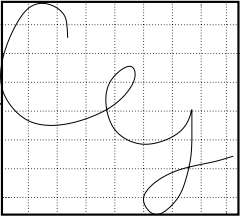
\includegraphics[scale=0.55]{pics/review/doodle.png}
        \label{fig:doodle}
      }
      \subfigure[CHC \cite{Wiedenbeck}]{
        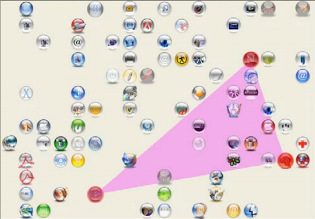
\includegraphics[scale=0.55]{pics/review/CHC.png}
        \label{fig:chc}
      }
    \end{figure}
    
  In 2007, Tao and Adams \cite{Tao} designed the graphical password scheme "Pass-Go". The creation of the scheme was motivated by one of the issues with the DAS scheme where it is difficult to accurately recreate the drawing. "Pass-Go" reduced the issue by using grid intersection points instead of grid cells as used in DAS. The users movements are captured into grid-lines and intersections, eliminating the possibility to reproduce a password where the difference is too high because of the need of precision in DAS. Figure~\ref{fig:passgo} is an image of the Pass-Go grid used.

  Out of the schemes mentioned until now are not widely known nor widely used by users. The first known graphical password scheme that have gained increased attention is the Android Unlock patten. The Android Unlock pattern is a mini version of the ``Pass-Go'' deployed on Google Android smartphones. Rather than entering a four-digit PIN or a text-based password, the user enters a touch-drawn password on a $3\times3$ grid connecting dots forming a password. Figure~\ref{fig:android} is a visualization of the Android Unlock Pattern in use on a smartphone.

    \begin{figure}[H]
      \centering
      \subfigure[Pass-go \cite{Tao}]{
        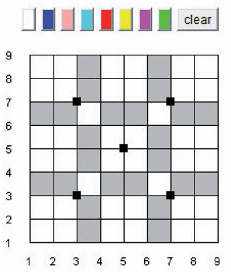
\includegraphics[scale=0.7]{pics/review/passgo2.png}
        \label{fig:passgo}
      }
      \subfigure[Android Unlock Pattern]{
        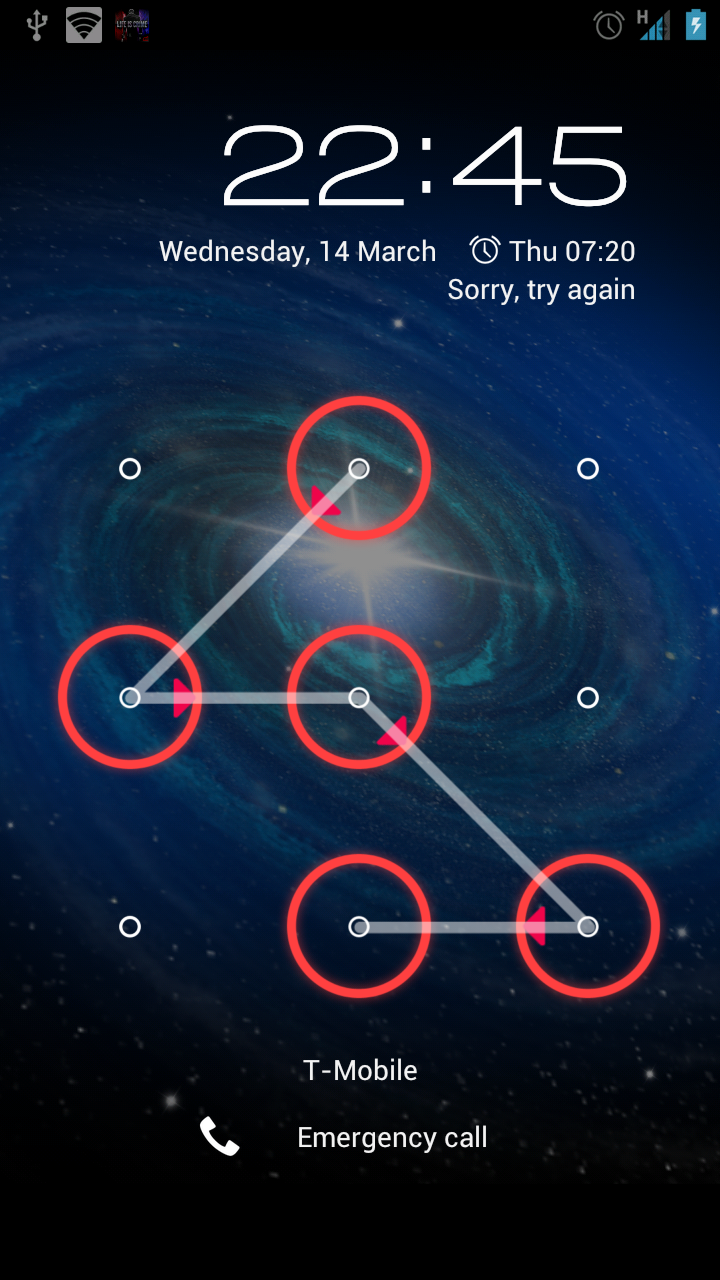
\includegraphics[scale=0.145]{pics/review/patternLock.png}
        \label{fig:android}
      }
    \end{figure}

  Looking at recently published graphical password schemes we will find schemes like GeoPass \cite{GeoPass} and Picassopass \cite{PicassoPass}. Geopass uses a digital map for the authentication phase where the user chooses a particular location as their password. Picassopass is a graphical password scheme presenting a password using a dynamic layered combination of graphical elements. The users can make a story that assists the user in the recognition of the graphical elements. Figure~\ref{fig:geopass} and Figure~\ref{fig:PicassoPass} is the two new proposals for graphical authentication schemes, the Geopass and the Picassopass, respectively. 

    \begin{figure}[H]
      \centering
      \subfigure[GeoPass \cite{GeoPass}]{
        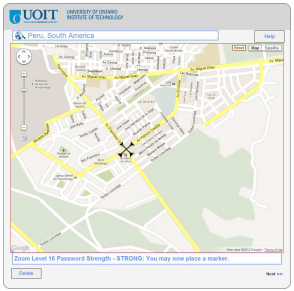
\includegraphics[scale=0.60]{pics/review/geopass.png}
        \label{fig:geopass}
      }
      \subfigure[PicassoPass \cite{PicassoPass}]{
        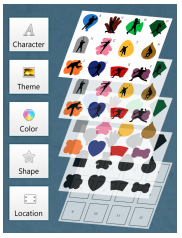
\includegraphics[scale=0.74]{pics/review/picassopass.png}
        \label{fig:PicassoPass}
      }
      \caption{Graphical password schemes}
    \end{figure}
  